

\subsection{Type of Backlash}



\subsection{Persistence}


We examine whether the location of refugee camps predicts where Spanish refugees ultimately settled after the Second World War, using data covering the universe of asylum applicants after 1945—approximately 160,000 individuals. Table~4 documents a strong and robust relationship between the presence of a refugee camp and subsequent refugee settlement. Across alternative functional forms, the coefficient on Camp remains positive and statistically significant. These results indicate that camps did not merely generate short-lived exposure to displaced populations but translated into persistent local settlement. This supports a demographic channel whereby refugee camps altered the composition of the local population, partially explaining the persistence of the political effects. As shown in \Cref{fig:refugees}, it also explains spillovers into control municipalities, as the relationship decreases with distance to the camp but remains statistically significant.

\begin{table}
\centering
\caption{Relationship between the refugees and the camps}
\centering
\begin{tabular}[t]{lcccc}
\toprule
  & (1) & (2) & (3) & (4)\\
\midrule
Within 1 km & 11.487 & 0.627*** & 0.422*** & 0.753***\\
\bottomrule
\multicolumn{5}{l}{\rule{0pt}{1em}* p $<$ 0.05, ** p $<$ 0.01, *** p $<$ 0.001}\\
\multicolumn{5}{l}{\rule{0pt}{1em}Column (1): OLS with fixed effects; column (2): ln.}\\
\multicolumn{5}{l}{\rule{0pt}{1em}Column (3): Poisson regression. Column (4): IHS / asinh}\\
\end{tabular}
\end{table}


\begin{table}
\centering
\caption{Characteristics of the refugees}
\centering
\begin{tabular}[t]{lcccccc}
\toprule
  & Left & No-left & High-skilled & Low-skilled & Nat & No Nat\\
\midrule
Camp & 0.390*** & 0.657*** & 0.486*** & 0.528*** & 0.314*** & 0.638***\\
\bottomrule
\multicolumn{7}{l}{\rule{0pt}{1em}* p $<$ 0.05, ** p $<$ 0.01, *** p $<$ 0.001}\\
\end{tabular}
\end{table}


\begin{figure}[htbp]
  \centering
  \caption{Relationship between refugee camps and refugees}
  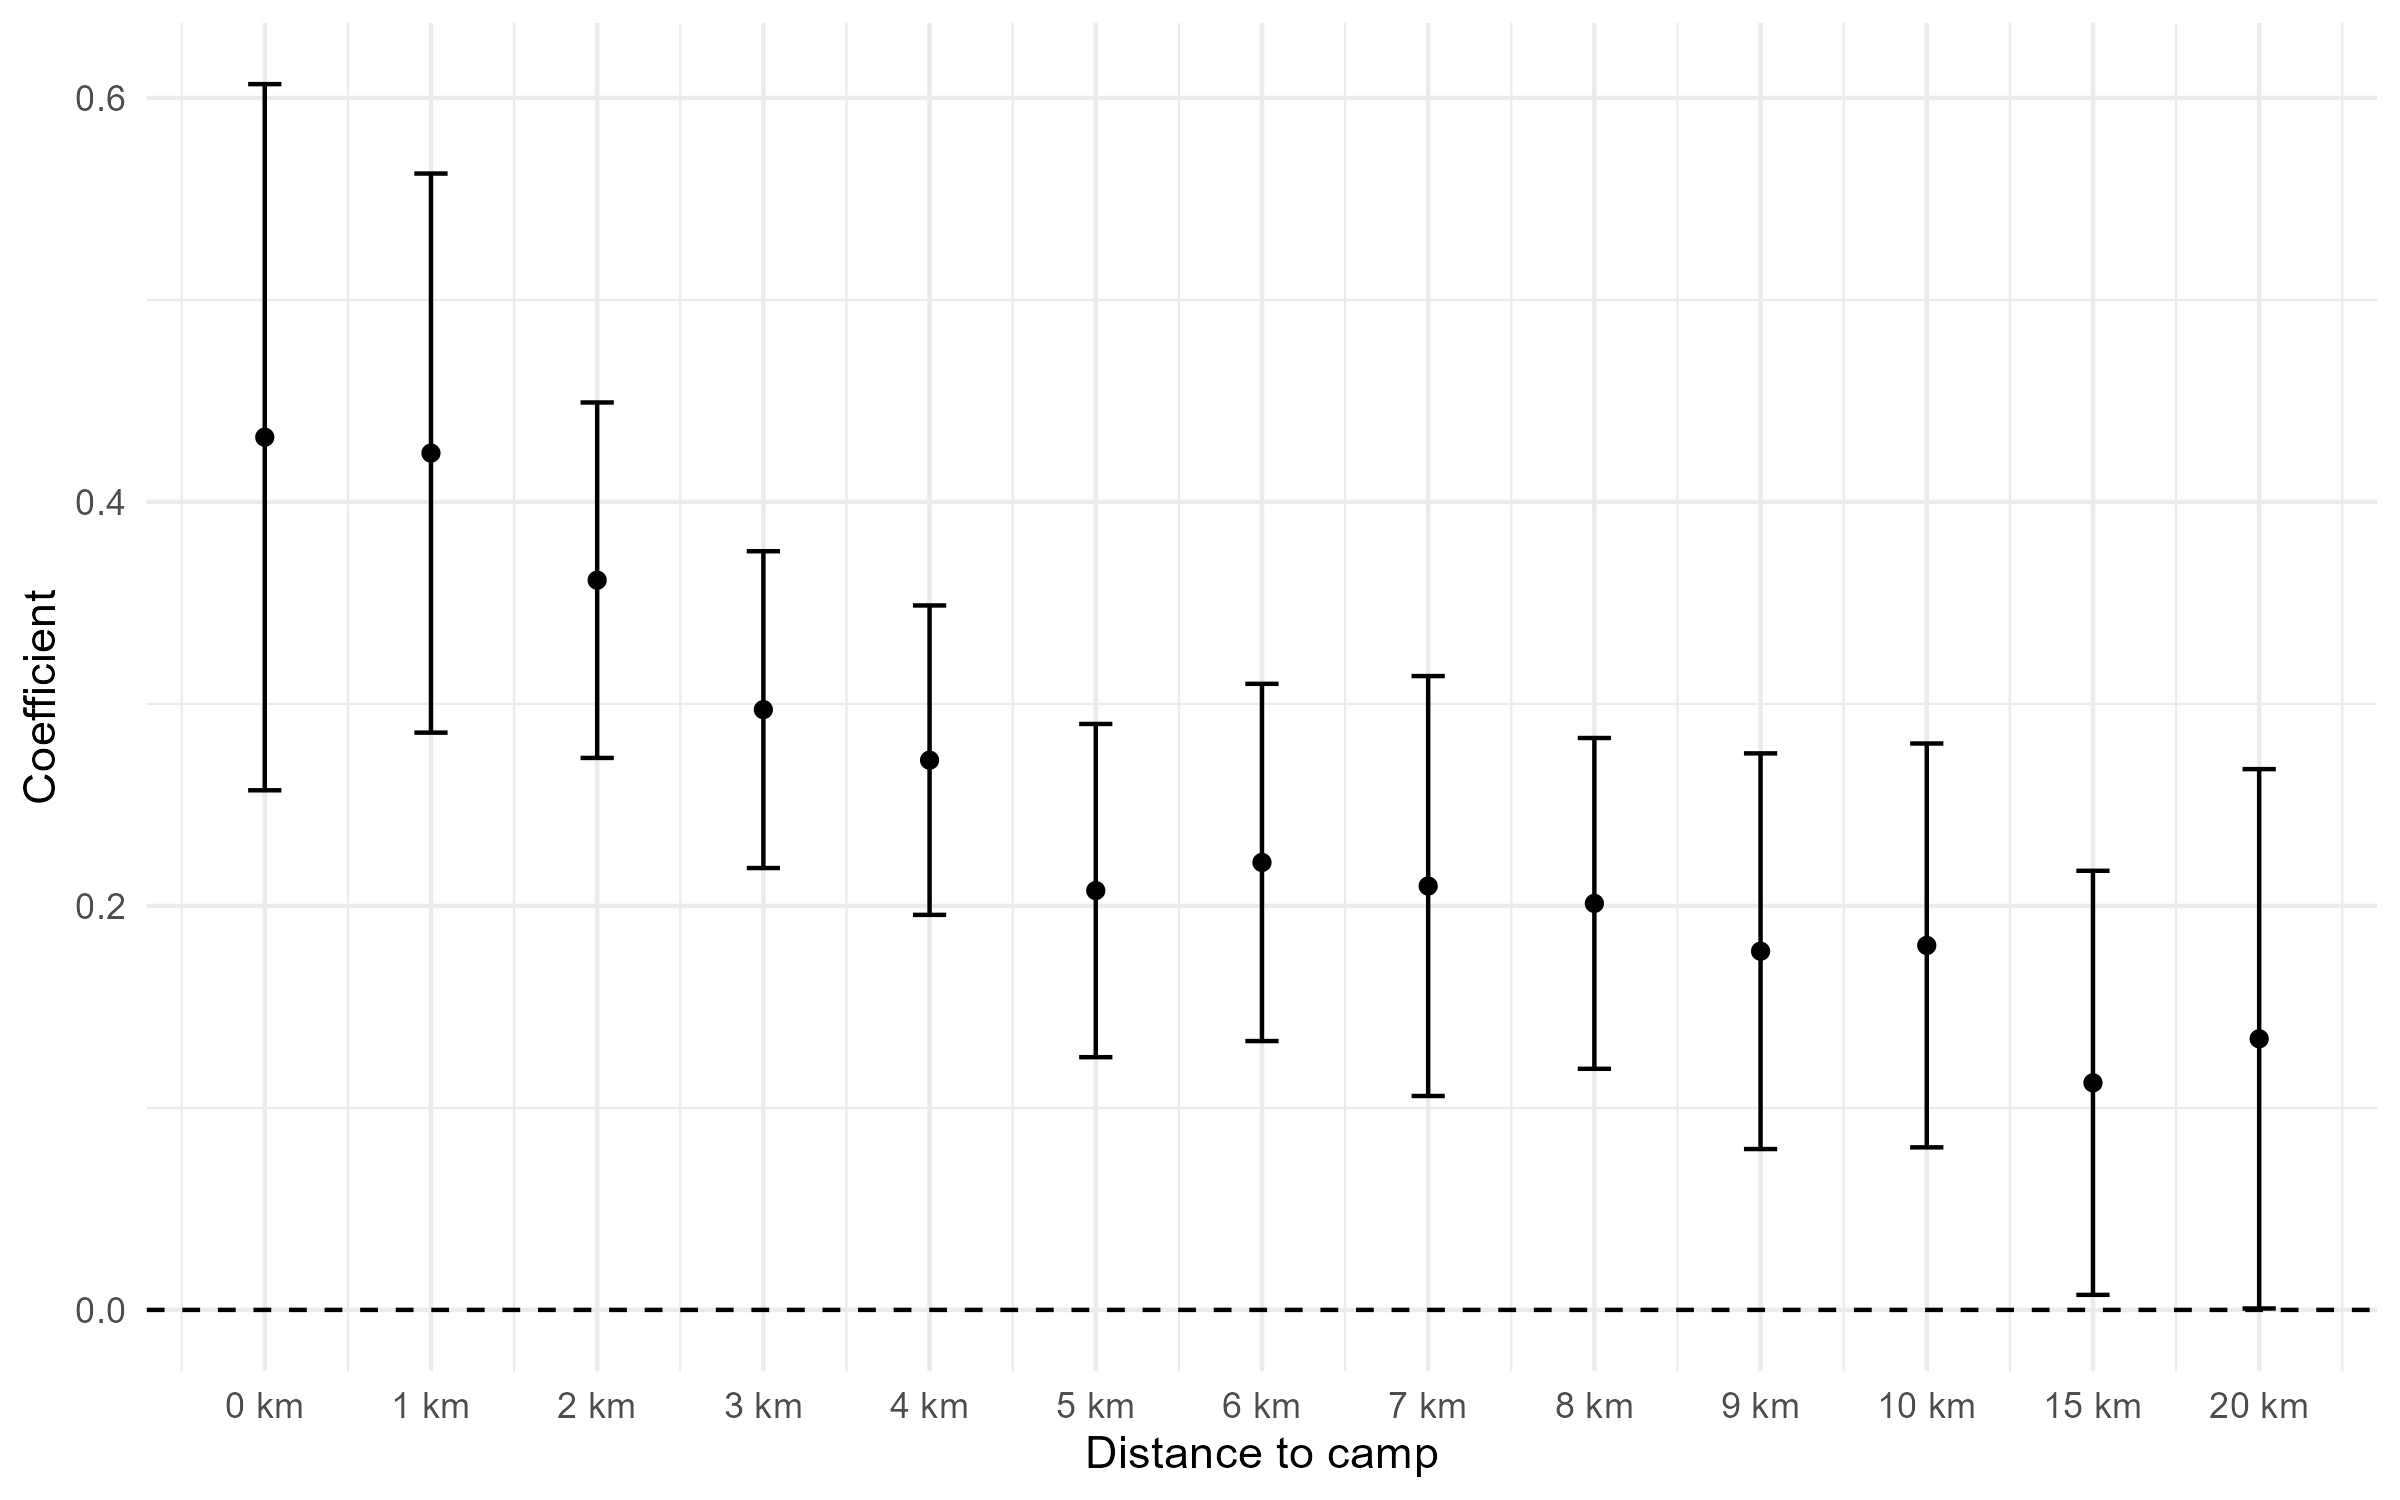
\includegraphics[width=0.8\linewidth]{figures/mechanisms/refugees_poisson.png}
  \label{fig:refugees}
   \begin{minipage}{0.7\textwidth}
        \vspace{0.5em}
        {\footnotesize Notes: This graph reports the estimates of Poisson regressions on the number of refugees after 1945. Standard errors are clustered to account for spatial correlation using \citet{conley_gmm_1999} (100 km). All specifications include department fixed effects and a set of controls—surname-based birthplace composition, altitude, mining activity, buildings per capita, average rainfall and the share of votes for the political parties of the 1936 legislative elections —and include a population offset.\par}
        \end{minipage}
\end{figure}




The results cannot be attributed to the electoral behaviour of the Spanish Republican refugees themselves. Legislative suffrage was restricted to French nationals, and the Vichy regime had dismantled the pre-war naturalization regime. Following the Liberation, the Ordinance of 19 October 1945 imposed a five-year residence requirement for naturalization, with eligibility additionally granted upon reaching majority after residing in France since age sixteen, or through marriage to a French national—although only 15\% of Spanish marriages between 1945 and 1950 were mixed \citep{Angoustures1997}. Code of 19 October 1945 also waived the residency requirement for volunteer enlistees, veterans of the two wars and members of the Resistance. Considering this framework, merely 6,400 Spaniards acquired the French nationality in 1946 \citep{spire_thave_1999}. Until 1978, slightly more than 15000 of Spanish refugees registered with the French Office for the Protection of Refugees acquired French nationality \citep{siglo_inmigracion_2009}. Moreover, newly naturalized individuals remained subject to legal incapacities: they were excluded from the electoral rolls for five years after naturalization and barred from holding elected office for ten years \citep{code_nationalite_fr_1945}. For these reasons, the settlement of Spanish refugees could not have mechanically translated into direct electoral participation.